\documentclass[lettersize,journal]{IEEEtran}
\usepackage{amsmath,amsfonts}
\usepackage{algorithmic}
\usepackage{algorithm}
\usepackage{array}
\usepackage[caption=false,font=normalsize,labelfont=sf,textfont=sf]{subfig}
\usepackage{textcomp}
\usepackage{stfloats}
\usepackage{url}
\usepackage{verbatim}
\usepackage{graphicx}
\usepackage{cite}
\usepackage{tikz}
\usepackage{pgf-pie}
\hyphenation{op-tical net-works semi-conduc-tor IEEE-Xplore}
% updated with editorial comments 8/9/2021

\begin{document}

\title{Pengetahuan dan Kemampuan yang Dimiliki Pengguna Non-Ahli dalam Mendeteksi Phishing}

\author{IEEE Publication Technology,~\IEEEmembership{Adhi Wahyu Utama and Dimas Anwar Aziz,~Telkom University,}
  % <-this % stops a space
  \thanks{This paper was produced by the IEEE Publication Technology Group. They are in Piscataway, NJ.}% <-this % stops a space
  \thanks{Manuscript received April 19, 2021; revised August 16, 2021.}
}

% The paper headers
\markboth{Journal of \LaTeX\ Class Files,~Vol.~14, No.~8, August~2021}%
{Shell \MakeLowercase{\textit{et al.}}: A Sample Article Using IEEEtran.cls for IEEE Journals}

% \IEEEpubid{0000--0000/00\$00.00~\copyright~2021 IEEE}
% Remember, if you use this you must call \IEEEpubidadjcol in the second
% column for its text to clear the IEEEpubid mark.

\maketitle

\begin{abstract}
  Email phishing adalah komunikasi penipuan yang berpura-pura menjadi sesuatu
  yang bukan sebenarnya untuk membuat orang melakukan tindakan yang seharusnya
  tidak mereka lakukan. Kami melakukan survei terhadap beberapa orang dari
  berbagai demografi di Indonesia dan meminta mereka untuk berbagi pengalaman
  mereka terkait email phishing. Dari analisis pengalaman tersebut, kami menemukan
  bahwa cara pengguna email mendeteksi pesan phishing memiliki banyak kesamaan
  dengan cara ahli IT mengidentifikasi phishing. Kami juga menemukan bahwa pengguna
  email memiliki pengetahuan unik dan kemampuan berharga dalam proses identifikasi
  yang tidak dimiliki oleh kontrol teknis maupun ahli IT. Kami menyarankan bahwa
  pelatihan yang ditargetkan pada cara memanfaatkan keunikan ini kemungkinan akan
  meningkatkan pencegahan phishing.
\end{abstract}

\begin{IEEEkeywords}
  Phishing detection, non-expert users, email security, user capabilities, cybersecurity awareness, security training, user knowledge, online threats, digital literacy, human factors in security.
\end{IEEEkeywords}

\section{Introduction}
\IEEEPARstart{E}{mail} adalah salah satu metode komunikasi yang paling umum
digunakan, terutama dalam organisasi besar dan e-commerce. Lebih dari 3,9 miliar
orang memiliki akun email, dan secara kolektif mereka mengirim dan menerima
lebih dari 290 miliar email per hari \cite{satusatu}. Email merupakan salah
satu metode utama yang digunakan untuk berkomunikasi dengan orang asing.
Namun, karena email adalah sistem global di mana siapa saja dapat berkomunikasi
dengan siapa saja, pelaku kejahatan mengirim email yang berpura-pura menjadi
sesuatu yang bukan sebenarnya, dan menipu orang untuk melakukan tindakan yang
seharusnya tidak mereka lakukan — yang dikenal sebagai phishing \cite{tigaempat}.
Pesan phishing adalah vektor serangan yang telah menyebabkan banyak kerugian
dalam masyarakat. Email phishing telah digunakan untuk mencuri uang dalam jumlah
besar \cite{duadua}, menginstal ransomware \cite{tigasatu}, atau sekadar mencuri
konten email yang kemudian dipublikasikan \cite{duasatu}. 32\% dari semua
pelanggaran perusahaan pada tahun 2018 disebabkan oleh phishing \cite{tigatiga}.
Spear-phishing – varian di mana email disesuaikan khusus dengan penerima – digunakan
oleh 65\% kelompok yang melakukan serangan siber yang ditargetkan, dan lebih umum
digunakan daripada kerentanan zero-day (hanya 23\% dari kelompok tersebut) \cite{tigadua}.

Phishing adalah masalah sosio-teknis, dan menangani masalah ini membutuhkan
kerja sama antara inovasi teknologi dan intervensi manusia. Teknologi sedang
dikembangkan untuk membantu mengidentifikasi dan menyaring pesan phishing,
tetapi teknologi ini tidak bekerja dengan akurasi 100\% dan dapat lambat
merespons inovasi baru oleh penyerang \cite{satuempat}. Administrator IT dan
pemerintah sering mencoba menghentikan phishing sebelum dimulai dengan
mengganggu situs web phishing dan pengiriman email massal \cite{satunol}.
Tetapi garis pertahanan terakhir adalah pengguna akhir; pesan phishing yang
melewati pertahanan lain masih dapat dideteksi atau diabaikan oleh pengguna
akhir untuk mencegah kerugian.

Dalam penelitian ini, kami mensurvei pengguna email tanpa pelatihan atau
keahlian IT dan menanyakan mereka tentang pengalaman spesifik dengan email
phishing yang mereka terima. Berdasarkan model Wash \cite{tigaempat} tentang
bagaimana ahli IT mendeteksi email phishing, kami menanyakan setiap orang
tentang apa yang mereka perhatikan dari email tersebut, apa yang mereka
harapkan dalam email tersebut, apa yang membuat mereka curiga terhadap email
tersebut, investigasi apa yang mereka lakukan, bagaimana mereka memutuskan
apakah email tersebut sah, dan apa yang akhirnya mereka lakukan dengan email
tersebut.

Dari pertanyaan-pertanyaan ini, kami dapat mengidentifikasi pola bagaimana
pengguna email yang bukan ahli IT saat mengidentifikasi email penipuan phishing
di kotak masuk mereka. Sebagian besar penelitian melihat kegagalan deteksi
phishing dan apa yang perlu diperbaiki; sebaliknya kami membandingkan non-ahli
dengan para ahli menurut Wash dan mengidentifikasi apa yang berhasil dengan
baik yang dapat kita kembangkan. Kami menemukan bahwa pengguna email sering
membawa pengetahuan unik ke proses identifikasi ini yang tidak dimiliki oleh
metode pencegahan phishing lainnya, seperti apakah email tersebut diharapkan
atau tidak dan seperti apa email seperti ini biasanya terlihat dan meminta.
Kami juga menemukan bahwa pengguna email memiliki kemampuan untuk investigasi,
seperti meminta saran dari orang lain, atau memeriksa keabsahan dengan
pengirim. Secara keseluruhan, temuan ini menunjukkan bahwa pengguna email dapat
menjadi bagian penting dari ekosistem pencegahan phishing, meskipun pelatihan
phishing dapat ditingkatkan untuk fokus pada bagaimana pengguna dapat
menggunakan pengetahuan dan kemampuan unik mereka dengan lebih baik.

\section{Previous Work}

\subsection{Mencegah Bahaya dari Phishing}
Masyarakat kita memiliki tiga bentuk pertahanan yang membantu mengidentifikasi
dan membatasi keberhasilan penipuan phishing. Pertahanan teknologi mencoba
secara otomatis mendeteksi fitur-fitur yang diketahui dari email phishing dan
memblokir atau menghapus email tersebut. Beberapa pertahanan menggabungkan
kerja komputer dan manusia dengan memperingatkan pengguna akhir tentang potensi
pesan phishing, yang kemudian diselidiki lebih lanjut oleh pengguna akhir untuk
menentukan apakah itu email phishing. Dan akhirnya, ada pertahanan manusia, di
mana penerima email diandalkan untuk mengenali email sebagai email berbahaya dan
bertindak untuk mengantisipasinya.

\subsubsection{Deteksi dan Penghapusan Otomatis}
Pendekatan deteksi dan penghapusan otomatis bertujuan untuk mengklasifikasikan
email sebagai phishing atau sah dan memblokir atau menghapusnya sebelum
pengguna akhir menemukannya. Upaya di bidang ini telah difokuskan pada
peningkatan dan menemukan cara baru untuk mengidentifikasi pesan phishing yang
masuk dan keluar menggunakan daftar hitam \cite{satunol}, heuristik [3, 13, 16,
    23], dan pembelajaran mesin [9, 29]. Pendekatan ini menyaring email berdasarkan
fitur yang diketahui yang secara konklusif mengidentifikasi email sebagai
phishing. Namun, pendekatan otomatis mengandalkan algoritma probabilistik yang
menghasilkan peringatan positif palsu, menyebabkan email sah diblokir atau dihapus. Selain
itu, pendekatan otomatis memiliki kemampuan terbatas untuk mendeteksi variasi
baru dari serangan phishing \cite{satudua} dan tidak dapat mengidentifikasi
semua email phishing yang lebih lama.

\subsubsection{Peringatan Phishing}
Peringatan phishing melengkapi teknik deteksi otomatis dengan memperingatkan
pengguna akhir tentang potensi email phishing, alih-alih memblokir atau
menghapusnya. Peringatan biasanya digunakan ketika deteksi otomatis tidak dapat
secara konklusif mengklasifikasikan email sebagai phishing \cite{dualima}.
Dalam praktiknya, peringatan telah dilaporkan meningkatkan kemampuan pengguna
akhir untuk mengidentifikasi email phishing [8, 26]. Upaya penelitian yang
sedang berlangsung di area ini telah difokuskan pada menemukan cara yang lebih
baik untuk merancang dan menyajikan peringatan kepada pengguna akhir.

Meskipun memiliki dampak positif, peringatan memiliki keterbatasan yang sama
dengan pendekatan deteksi dan penghapusan otomatis. Mereka rentan terhadap
peringatan positif palsu (menandai email sah sebagai berpotensi berbahaya) dan
peringatan negatif palsu (membiarkan email berbahaya lolos tanpa peringatan,
terutama serangan phishing zero-hour). Seperti yang dikemukakan oleh Yang et
al., peringatan dan pelatihan pengguna harus saling melengkapi untuk
meningkatkan efektivitasnya \cite{tigatujuh}.

\subsubsection{Pelatihan Pengguna}
Peneliti dan praktisi keamanan telah mengembangkan berbagai metode dan materi
untuk melatih pengguna mengidentifikasi dan bereaksi terhadap email phishing
dengan tepat. Kumaraguru et al. \cite{satusembilan} dan Caputo et al.
\cite{dua} menemukan bahwa pelatihan tertanam (yaitu materi instruksional yang
disajikan saat peserta mengklik URL dalam email phishing), yang sangat umum
digunakan di organisasi besar, meningkatkan motivasi pengguna untuk belajar dan
meningkatkan akuisisi pengetahuan. Rader et al. \cite{duatujuh} menemukan bahwa
orang juga belajar tentang penipuan phishing dan tindakan perlindungan dari
cerita tentang insiden keamanan. Wash dan Cooper \cite{tigalima} menemukan
bahwa pelatihan phishing tradisional yang berisi fakta dan saran bekerja lebih
baik ketika disajikan oleh seorang ahli, sementara cerita keamanan naratif
bekerja lebih baik ketika diceritakan oleh seorang rekan.

Pesan pelatihan phishing yang paling banyak dibagikan di seluruh pemerintah,
bisnis, dan individu mengajarkan orang untuk mengidentifikasi tanda-tanda
tertentu (misalnya alamat email pengirim, URL dalam email, tata bahasa atau
ejaan yang buruk) atau menerapkan serangkaian aturan untuk mendeteksi,
menghindari, dan melaporkan pesan phishing. Pesan pelatihan semacam itu telah
dipelajari secara ekstensif dan menunjukkan potensi untuk meningkatkan
ketahanan orang terhadap serangan phishing [4, 19]. Beberapa pesan berfokus
pada perubahan perilaku, misalnya, tidak pernah mengklik URL atau membuka
lampiran dalam email dari pengirim yang tidak dikenal.

Pesan pelatihan lainnya berfokus pada memberi tahu pengguna tentang jenis
ancaman phishing yang umum dan cara mengidentifikasinya, dengan tujuan
memanipulasi tingkat risiko dan selanjutnya tingkat ketakutan pada pengguna [5,
    20]. Beberapa peneliti berpendapat bahwa ajakan ketakutan meningkatkan niat
pengguna akhir untuk bertindak dengan aman. Namun, meskipun mampu mengubah niat
perilaku pengguna akhir \cite{lima}, ajakan ketakutan tidak memprediksi atau
menghasilkan perilaku yang aman \cite{enam}.

Pelatihan pengguna biasanya berfokus pada aspek pesan email dan mencoba
mengubah cara orang berpikir tentang pesan email sehingga mereka memperhatikan
fitur yang paling terkait dengan phishing. Studi telah menunjukkan bahwa ini
meningkatkan pengetahuan pengguna, meningkatkan kemampuan mereka untuk
mengidentifikasi email phishing, dan mengurangi jumlah serangan yang berhasil
  [2, 19, 35]. Namun, jumlah serangan phishing yang berhasil masih cukup tinggi,
mencapai 32\% dari semua pelanggaran perusahaan pada tahun 2018. Masih banyak
yang perlu dilakukan untuk meningkatkan kemampuan pengguna akhir dalam
mengidentifikasi dan mencegah serangan phishing.

Sebagian besar pelatihan pengguna dikembangkan dari pemahaman tentang bagaimana
dan mengapa orang jatuh ke dalam phishing \cite{enam}. Kami berhipotesis bahwa
jika pelatihan lebih fokus pada aspek bagaimana orang berpikir tentang email
dan menangani email secara umum, ini dapat membuka jalan baru untuk pelatihan
phishing. Sayangnya, kami tidak memiliki pemahaman yang komprehensif tentang
bagaimana pengguna non-ahli melakukannya. Masalah serupa dihadapi dalam
pelatihan keterampilan teknis di mana peneliti menyelidiki cara untuk
meningkatkan pelatihan pemecahan masalah (teknisi) \cite{satulima}. Mereka
mempelajari dan mengidentifikasi proses konseptual umum dan strategi yang
digunakan teknisi saat memecahkan masalah. Ini membantu mereka mengidentifikasi
kesenjangan dalam metode dan pesan pelatihan yang ada dan selanjutnya membantu
mereka mengidentifikasi area perbaikan. Kami berpendapat bahwa memahami proses
dan strategi yang digunakan non-ahli untuk mengidentifikasi email phishing
dapat mengungkapkan area potensial untuk perbaikan pelatihan phishing.

\subsection{Bagaimana Orang Mengidentifikasi Email Phishing?}

Downs et al. \cite{tujuh} menyelidiki strategi keputusan pengguna komputer
non-ahli ketika menghadapi email yang mencurigakan. Mereka mengidentifikasi
tiga strategi yang digunakan peserta untuk memahami email yang mereka terima:
1) email ini tampaknya ditujukan untuk saya; 2) normal untuk mendengar dari
perusahaan yang Anda lakukan bisnis dengannya dan 3) perusahaan terkemuka akan
mengirim email. Downs et al. \cite{tujuh} menyatakan bahwa tidak ada strategi
yang membantu orang mengidentifikasi pesan phishing yang dirancang dengan baik.
Namun, studi tersebut melibatkan peran bermain dalam lingkungan yang
terkendali. Kami tidak tahu strategi mana yang berlaku dan seberapa umum mereka
dalam konteks alami dan kotak masuk orang.

Wash \cite{tigaempat} melihat bagaimana ahli mengidentifikasi email phishing
dengan mewawancarai 21 ahli IT tentang kejadian ketika mereka berhasil
mengidentifikasi email sebagai phishing di kotak masuk mereka. Dia
mengidentifikasi proses 3 tahap untuk mengidentifikasi email phishing. Pada
tahap pertama, email diterima dan diperlakukan seperti email lainnya — konten
dalam email diambil secara harfiah dan orang tersebut mencoba memahami email
dan mencari tahu apa yang diminta untuk dilakukan. Saat mereka melakukan ini,
mereka memperhatikan ketidaksesuaian — hal-hal yang "terasa aneh" tentang email
tersebut. Akhirnya, sesuatu memicu orang tersebut untuk berpikir bahwa email
ini tidak sah — bahwa itu mungkin email phishing yang bukan seperti yang
dikatakannya. Pada titik ini, mereka menjadi curiga dan mulai secara eksplisit
mencari hal-hal yang dapat membantu mereka menentukan apakah email tersebut sah
atau tidak. Potongan informasi baru ini sering memungkinkan mereka untuk secara
konklusif mengidentifikasi email sebagai phishing.

Pekerjaan Wash \cite{tigaempat} menunjukkan bagaimana beberapa pelajaran dari
pelatihan phishing diterapkan dalam konteks dunia nyata. Namun, Wash hanya
mempelajari para ahli. Para ahli mungkin memiliki keterampilan, pengalaman, dan
pengetahuan yang lebih maju tentang phishing dan tindakan pencegahan
dibandingkan dengan non-ahli. Kami tidak tahu temuan mana yang mungkin berlaku
untuk non-ahli dan dapat digunakan untuk meningkatkan pelatihan mereka.

\subsection{Phishing: Masalah Sosio-Teknis}

Phishing adalah masalah sosio-teknis. Solusi otomatis tidak mendeteksi 100\%
email phishing. Oleh karena itu, pengguna akhir harus mengidentifikasi email
ini di kotak masuk mereka. Seperti yang dikatakan oleh Khonji et al., tidak ada
solusi tunggal yang ada untuk mengurangi serangan phishing \cite{satutujuh};
sehingga teknik otomatis / peringatan dan pelatihan pengguna harus diterapkan
untuk saling melengkapi \cite{satusembilan}. Ini sebanding dengan Model Keju
Swiss (SCM) James Reason \cite{duadelapan} tentang penyebab dan respons
kecelakaan. SCM adalah alat populer yang digunakan untuk menyelidiki atau
menganalisis kompleksitas sistem dengan menunjukkan bahwa suatu insiden adalah
hasil dari kombinasi kegagalan aktif oleh operator dan kondisi laten dari
sistem. SCM menggambarkan sistem sosio-teknis sebagai beberapa irisan keju
Swiss yang ditumpuk bersama, masing-masing irisan dengan lubang. Setiap irisan
menggambarkan lapisan pertahanan sistem terhadap jenis kegagalan tertentu,
sementara setiap lubang mewakili kegagalan dalam pertahanan sistem pada lapisan
tertentu. Bryans dan Arief menerapkan model tersebut untuk memahami lapisan
keamanan dan toleransi kesalahan dalam sistem komputer \cite{satu}. Mereka
menggambarkan setiap lapisan sebagai mekanisme perlindungan terhadap jenis
serangan tertentu, tetapi memiliki kelemahan (lubang) terhadap jenis lainnya.

Baik teknik deteksi dan penghapusan otomatis maupun peringatan mengandalkan
pengguna akhir sebagai garis pertahanan terakhir terhadap phishing. Namun,
jumlah serangan phishing yang berhasil baru-baru ini menunjukkan bahwa lebih
banyak hal perlu dilakukan untuk meningkatkan pelatihan pengguna. Sementara
sebagian besar pelatihan berfokus pada mengajarkan pengguna akhir untuk
mengidentifikasi fitur yang diketahui dan konklusif dari email phishing, Downs
et al. \cite{tujuh} dan Wash \cite{tigaempat} menemukan bahwa pengguna akhir
mengandalkan fitur selain pembeda konklusif untuk mengidentifikasi email
phishing. Kita perlu mengeksplorasi cara-cara yang lebih baik untuk menjaga
pengguna dalam lingkaran pertahanan terhadap serangan phishing. Lebih banyak
penelitian perlu dilakukan untuk memahami bagaimana non-ahli mengidentifikasi
email phishing, aspek atau informasi apa yang mereka andalkan, dan jenis hal
yang mereka lakukan dalam proses tersebut. Pemahaman ini dapat membantu kita
menyesuaikan dan menargetkan pelatihan phishing dan teknologi yang mendukung
pengambilan keputusan manusia. Studi kami mengambil langkah pertama ke arah ini
dengan menerapkan model Wash dalam survei untuk mempelajari teknik yang diikuti
non-ahli untuk mengidentifikasi email phishing.

\section{Methods and Sample}

Dalam makalah ini, kami melihat bagaimana pengguna non-ahli di Indonesia
mengidentifikasi email phishing, dan melihat apakah beberapa teknik yang
diidentifikasi oleh Wash \cite{tigaempat} pada ahli juga ada ketika non-ahli
mengidentifikasi email phishing. Untuk mempelajari ini, kami melakukan survei
di mana kami meminta pengguna internet non-ahli untuk mengingat email tertentu
yang mereka terima yang "mencurigakan atau berpotensi berbahaya," dan kemudian
menjawab pertanyaan tentang pengalaman mereka dengan email tersebut.

Kami mengajukan pertanyaan untuk mencoba memahami apa yang mereka perhatikan
dan tidak perhatikan tentang email yang diterima responden dan memahami hal-hal
apa yang tampaknya penting bagi mereka. Ini adalah catatan retrospektif tentang
email masa lalu; kami mengharapkan bahwa responden tidak akan mengingat
beberapa detail tentang apa yang terjadi. Kami membuat asumsi bahwa hal-hal
yang tidak mereka ingat kemungkinan besar kurang penting dalam pemikiran mereka
tentang email tersebut \cite{satudelapan}.

\subsection{Survei}
Kami memulai dengan instrumen survei yang didasarkan pada Wash et al.
\cite{ref10}. Kami membuat penyesuaian terhadap pertanyaan survey karena
pertimbangan waktu pelaksanaan penelitian. Kami tidak menyertakan pertanyaan
yang dijawab secara esay, yang kami gunakan adalah pertanyaan dengan jawaban
pilihan yaitu pertanyaan dengan 1 jawaban, beberapa jawaban, dan jawaban berupa
pilihan skala. Di awal survei, kami meminta responden untuk mengidentifikasi
"cerita" atau insiden tertentu di mana mereka menerima email yang mencurigakan
atau berpotensi berbahaya. Kami kemudian meminta mereka untuk menjawab sejumlah
pertanyaan tentang insiden tertentu tersebut.

Kami menyertakan pertanyaan penyaringan yang menanyakan kepada calon responden
apakah mereka dapat mengingat menerima jenis email yang kami minati. Survei
memberi tahu responden bahwa "Dalam survei ini, kami tertarik mendengar tentang
email yang Anda terima yang mencurigakan atau berpotensi berbahaya dengan cara
tertentu." Kemudian meminta mereka untuk mengingat kembali email mereka, dan
memberi tahu mereka bahwa tidak apa-apa untuk melihat kembali email mereka jika
itu akan membantu. Kami bertanya "Apakah Anda dapat mengingat pesan email yang
mencurigakan atau berpotensi berbahaya yang pernah Anda terima?" Hanya
responden yang menjawab ya untuk pertanyaan ini yang melanjutkan survei.

Berdasarkan model Wash [34], kami mengidentifikasi enam proses yang digunakan
para ahli dalam mendeteksi phishing. Kami menyusun pertanyaan di sekitar enam
proses ini:

\begin{enumerate}
  \item{Memperhatikan}: Hal-hal yang mereka perhatikan tentang email, seperti kapan mereka menerima email, jenis email (lampiran, dll.), konten kerja atau pribadi, akun kerja atau pribadi, dll.
  \item{Mengharapkan}: Apa yang mereka harapkan dalam email; membangun dari memperhatikan dan membandingkan apa yang mereka perhatikan dengan apa yang mereka harapkan. Apakah mereka pernah menerima email lain seperti ini, berinteraksi dengan pengirim sebelumnya, apakah email tersebut diharapkan, dll.
  \item{Mencurigai}: Apa yang terasa "aneh" tentang email — subjek, dari, isi, dll. Apa yang ada dalam email yang membuat mereka curiga terhadap email tersebut. Apakah itu berisi tautan, lampiran, dll.
  \item{Menyelidiki}: Apa yang mereka cari secara eksplisit setelah mereka mencurigai email tersebut (jika ada) untuk mengetahui apakah email tersebut sah atau penipuan. Hal-hal seperti "apakah Anda melihat header, atau mengarahkan kursor ke tautan, atau mencoba menghubungi pengirim?"
  \item{Memutuskan}: Bagaimana keputusan sah/phish dibuat. Apakah Anda memutuskan, dan jika ya, bagaimana? Seberapa yakin Anda?
  \item{Bertindak}: Setelah memutuskan, apa yang Anda lakukan dengan email tersebut? Melaporkannya? Hanya menghapusnya? Bagaimana perasaan Anda tentang email tersebut? Takut? Kecemasan? Kegelisahan?
\end{enumerate}

\subsection{Sampel}

Survey disebarkan melalui google form selama 2 minggu dan kami mendapatkan 64
tanggapan. Selanjutnya kami melakukan penyaringan pertama menggunakan
pertanyaan "Apakah Anda pernah menerima pelatihan formal dalam ilmu komputer,
rekayasa perangkat lunak, IT, jaringan komputer, atau bidang teknis terkait?",
hasilnya 18 responden (28\%) menjawab "Ya" dan 4 responden (6\%) menjawab "Saya
tidak yakin", sehingga kami mengeluarkan 22 sampel ini. Selanjutnya dilakukan
penyaringan kedua dengan pertanyaan "Apakah Anda pernah bekerja di pekerjaan
"teknologi tinggi" seperti pemrograman komputer, IT, atau jaringan komputer?",
hasilnya 1 responden (2\%) menjawab "Ya" sehingga data tersebut kami keluarkan.
Penyaringan terakhir adalah dengan pertanyaan "Apakah Anda ingat pesan email
mencurigakan atau berpotensi berbahaya yang pernah Anda terima? Anda boleh
memeriksa akun email Anda dan kemudian melanjutkan survei, untuk membantu Anda
mengingat apakah Anda pernah menerima pesan email seperti ini.". Hasilnya 8
responden (19\%) menjawab "Tidak, saya tidak ingat pernah menerima pesan email
seperti ini." dan 5 responden (12\%) menjawab "Saya tidak yakin", sehingga kami
mengeluarkan 13 data ini dari sampel. Hasil akhirnya didapat 28 data responden
valid.

Tabel 1 merangkum demografi sampel kami.

\begin{table*}[h!]
  \centering
  \caption{Demografi sampel survei. Kami menerima tanggapan yang valid dengan total 28 responden.}
  \begin{tabular}{@{}llrl@{}}
    \toprule
    \textbf{Kategori}                              & \textbf{Subkategori} & \textbf{N} & \textbf{\%} \\ \midrule
    \textbf{Usia}                                  & 15--24               & 2          & 7\%         \\
                                                   & 25--34               & 1          & 3\%         \\
                                                   & 35--44               & 13         & 47\%        \\
                                                   & 45 tahun ke atas     & 12         & 43\%        \\ \midrule
    \textbf{Jenis Kelamin}                         & Pria                 & 13         & 46\%        \\
                                                   & Wanita               & 15         & 54\%        \\   \midrule
    \textbf{Etnis}                                 & Jawa                 & 1          & 82\%        \\
                                                   & Betawi               & 1          & 3\%         \\
                                                   & Minangkabau          & 1          & 3\%         \\
                                                   & Melayu               & 1          & 3\%         \\
                                                   & Papua                & 1          & 3\%         \\
                                                   & Bugis                & 1          & 3\%         \\ \midrule
    \textbf{Pendidikan}                            & SMU                  & 3          & 10\%        \\
                                                   & D3                   & 1          & 3\%         \\
                                                   & S1                   & 14         & 50\%        \\
                                                   & S2/S3                & 10         & 35\%        \\ \midrule
    \textbf{Pekerjaan}                             & Bekerja Penuh Waktu  & 21         & 77\%        \\
                                                   & Bekerja Paruh Waktu  & 2          & 7\%         \\
                                                   & Pensiunan            & 2          & 7\%         \\
                                                   & Pelajar              & 2          & 7\%         \\ \midrule
    \textbf{Pendapatan Rumah Tangga Tahunan (USD)} & 2 juta ke bawah      & 3          & 11\%        \\
                                                   & antara 3 - 6 juta    & 3          & 11\%        \\
                                                   & antara 7 - 10 juta   & 9          & 33\%        \\
                                                   & antara 11 - 14 juta  & 4          & 14\%        \\
                                                   & antara 15 - 18 juta  & 3          & 11\%        \\
                                                   & diatas 18 juta       & 5          & 18\%        \\ \bottomrule
  \end{tabular}
\end{table*}

\subsection{Analisis}

\section{Findings}

\begin{figure}[h]
  \centering
  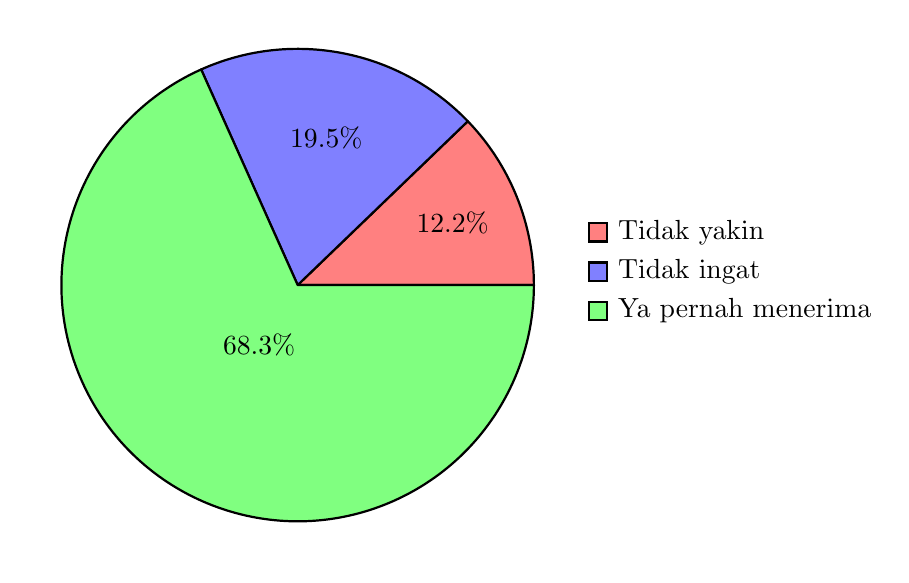
\begin{tikzpicture}
    \pie[
      text=legend,
      radius=3,
      color={red!50, blue!50, green!50}
    ]{
      12.2/Tidak yakin,
      19.5/Tidak ingat,
      68.3/Ya pernah menerima
    }
  \end{tikzpicture}
  \caption{Persentase Responden yang Pernah Menerima Email Phishing}
  \label{fig:phishing_experience}
\end{figure}

Dalam survei ini, kami meminta responden untuk mengidentifikasi "pesan email
yang mencurigakan atau berpotensi berbahaya yang Anda terima di masa lalu."
Dari 41 responden non IT, 28 responden (68\%) berhasil mengingat email ini.
Tujuan kami bukan untuk menemukan seberapa umum phishing di antara kelompok
demografis yang berbeda, dan sampel ini bukan sebagai pengukuran prevalensi
phishing. Namun, ini menunjukkan bahwa sekitar 68\% dari orang-orang non IT
memiliki cerita tentang email phishing tertentu yang mereka terima, yang
menunjukkan betapa luasnya pengalaman dengan email-email ini.

Hampir semua pertanyaan yang tersisa dalam survei kemudian meminta responden
untuk memberikan lebih banyak detail tentang insiden spesifik di mana mereka
menerima email yang mereka pilih untuk diceritakan kepada kami: apa yang
terjadi saat mereka menerimanya, apa yang mereka perhatikan, dan bagaimana
mereka menanganinya? Dalam sebagian besar makalah ini, kami melaporkan
statistik tentang tanggapan terhadap pertanyaan pilihan ganda.

Berdasarkan temuan dari Wash \cite{tigaempat}, kami mengorganisir survei
berdasarkan enam aktivitas berbeda yang perlu dilakukan seseorang untuk
mengenali email phishing: 1) Memperhatikan aspek-aspek email; 2) Membentuk
ekspektasi tentang apa yang seharusnya dan tidak seharusnya ada dalam email; 3)
Menjadi curiga terhadap email; 4) Menyelidiki email; 5) Memutuskan apakah email
mencurigakan atau tidak; dan 6) Bertindak berdasarkan keputusan tersebut.

Enam aktivitas ini memberikan cara bagi kami untuk menggambarkan apa yang
umumnya terjadi ketika seseorang menerima email phishing, dan untuk melihat
pola dalam apa yang mereka perhatikan dan apa yang mereka lakukan. Kami
mengorganisir deskripsi temuan kami dalam makalah ini di sekitar enam aktivitas
berbeda ini.

\subsection{Insiden}

Setiap peserta diminta untuk menjawab pertanyaan tentang satu insiden yang
mereka alami. Kami mulai dengan menggambarkan jenis insiden yang dilaporkan
oleh responden. Setiap insiden adalah email yang diterima peserta dan dianggap
mencurigakan atau berpotensi berbahaya. Semua insiden ini mewakili email yang
berhasil melewati pertahanan teknis dan masuk ke kotak masuk peserta, sehingga
tidak termasuk email phishing yang berhasil difilter oleh perlindungan phishing
teknis.

Sekitar 57\% responden menunjukkan bahwa mereka merasa mudah mengingat email
semacam itu.

\begin{figure}[h!]
  \centering
  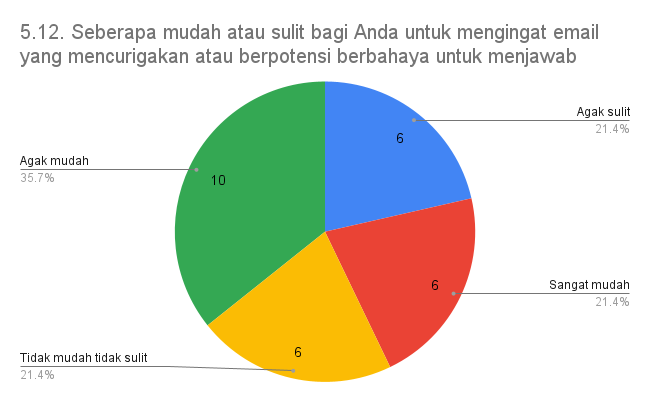
\includegraphics[width=0.5\textwidth]{image/5.12.png}
  \caption{hasil pertanyaan 5.12}
  \label{fig:pertanyaan_5.12}
\end{figure}

Email-email yang dipilih responden untuk dijawab tersebar luas dalam waktu: 7\%
responden menerimanya dalam minggu terakhir; 30\% dalam bulan terakhir (tetapi
bukan minggu terakhir); 42\% dalam tahun terakhir (tetapi bukan bulan
terakhir); dan 17\% lebih dari setahun yang lalu.

\begin{figure}[h!]
  \centering
  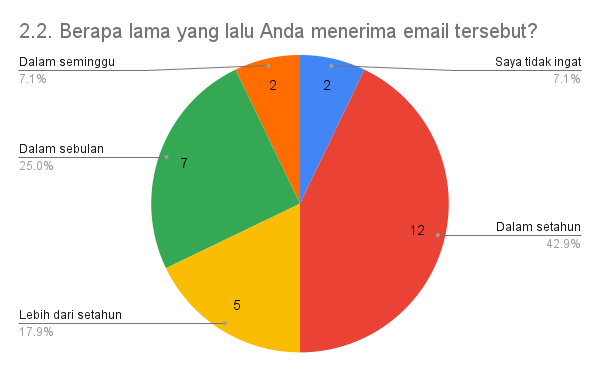
\includegraphics[width=0.5\textwidth]{image/2.2.png}
  \caption{hasil pertanyaan 2.2}
  \label{fig:pertanyaan_2.2}
\end{figure}



\subsection{Noticing}

Dalam memperhatikan aspek-aspek dari email, terdapat sejumlah aspek situasi 
yang sebenarnya bukan bagian dari email itu sendiri tetapi tetap dianggap penting dan berkesan oleh responden.

Sebanyak 64\% responden menyadari bahwa email tersebut masuk ke akun email
pribadi mereka, sedang 28\% responden menerima email tersebut di akun email pekerjaan. 
Hanya 1 responden (3\%) yang memilih opsi “Saya tidak ingat”
mengenai akun email tempat email itu diterima. Akun tempat email diterima 
tampaknya menjadi hal yang menonjol dan mudah diingat oleh responden, serta
kemungkinan dapat digunakan untuk membantu mengidentifikasi email yang mencurigakan. 

\begin{figure}[h!]
  \centering
  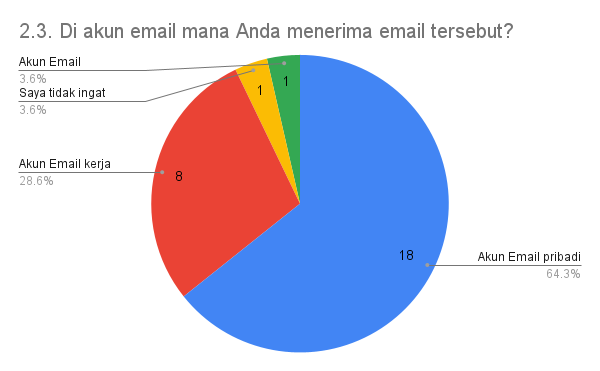
\includegraphics[width=0.5\textwidth]{image/2.3.png}
  \caption{hasil pertanyaan 2.3}
  \label{fig:pertanyaan_2.3}
\end{figure}

Mengenai konteks isi email, 35\% responden melaporkan bahwa email tersebut bersifat pribadi 
dan 28\% menyampaikan sifat email tersebut berhubungan dengan pekerjaan.
Cukup banyak responden yang tidak bisa mengingat konteks dari email yaitu 28\%.

\begin{figure}[h!]
  \centering
  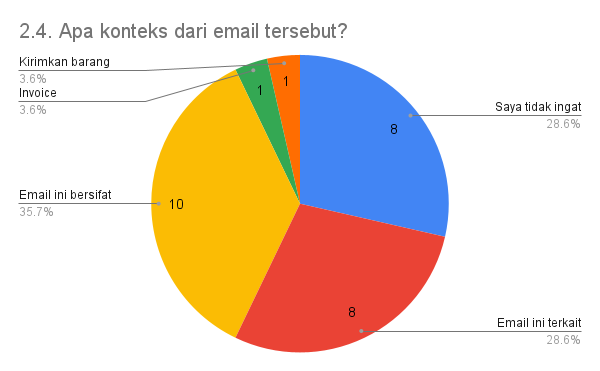
\includegraphics[width=0.5\textwidth]{image/2.4.png}
  \caption{hasil pertanyaan 2.4}
  \label{fig:pertanyaan_2.4}
\end{figure}

Tentang pengirim, sebanyak 78\% responden melaporkan bahwa email tersebut tampak berasal dari 
perusahaan, bisnis, atau organisasi lainnya. 7\% mengatakan email tersebut tampaknya berasal dari
orang asing, dan 7\% dari kenalan di luar pekerjaan. Kemudian
7\% responden tidak dapat mengingat dari siapa email itu tampaknya 
berasal. 

\begin{figure}[h!]
  \centering
  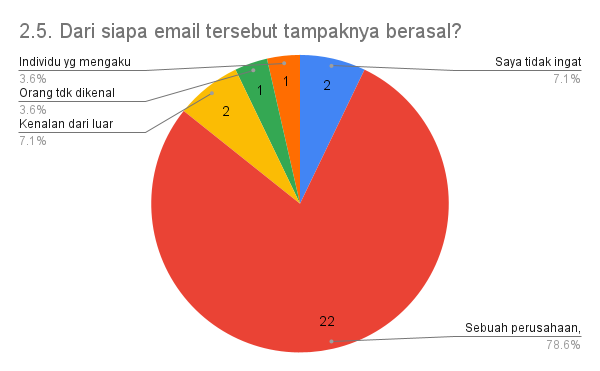
\includegraphics[width=0.5\textwidth]{image/2.5.png}
  \caption{hasil pertanyaan 2.5}
  \label{fig:pertanyaan_2.5}
\end{figure}

\subsection{Expecting}

Ketika mencoba memahami dan membuat penilaian tentang sebuah email, orang
secara alami kembali pada jenis email yang mereka harapkan untuk diterima, dan
membandingkan email tersebut dengan email-email sebelumnya yang pernah mereka
terima \cite{tigaempat}.

Hampir semua email mencurigakan tiba secara tidak terduga (82\%). Ini tampaknya
menjadi salah satu aspek terkuat dari identifikasi phishing bagi responden
kami. Ini juga sesuatu yang pengguna temukan relatif mudah untuk
diidentifikasi, tetapi hampir tidak mungkin diukur secara teknis. Artinya,
apakah sebuah email diharapkan atau tidak adalah sesuatu yang merupakan
informasi berharga yang hanya dimiliki oleh pengguna dan tidak dimiliki oleh
komputer.

\begin{figure}[h!]
  \centering
  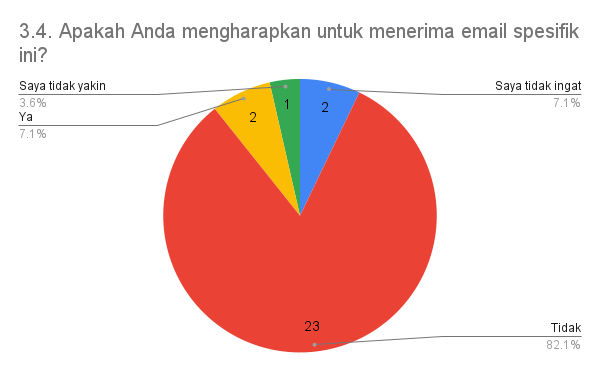
\includegraphics[width=0.5\textwidth]{image/3.4.png}
  \caption{hasil pertanyaan 3.4}
  \label{fig:pertanyaan_3.4}
\end{figure}

Walaupun email tersebut tidak diharapkan tidak berarti email
tersebut tidak familiar. 39\% responden melaporkan "agak setuju" atau "sangat
setuju" dengan pernyataan "Saya merasa seperti saya telah menerima pesan email
lain seperti ini sebelumnya." Artinya, lebih dari sepertiga email terasa
familiar bagi penerima. Responden yang tidak familiar mencapai 35\% dan 25\% 
responden menyatakan netral.

\begin{figure}[h!]
  \centering
  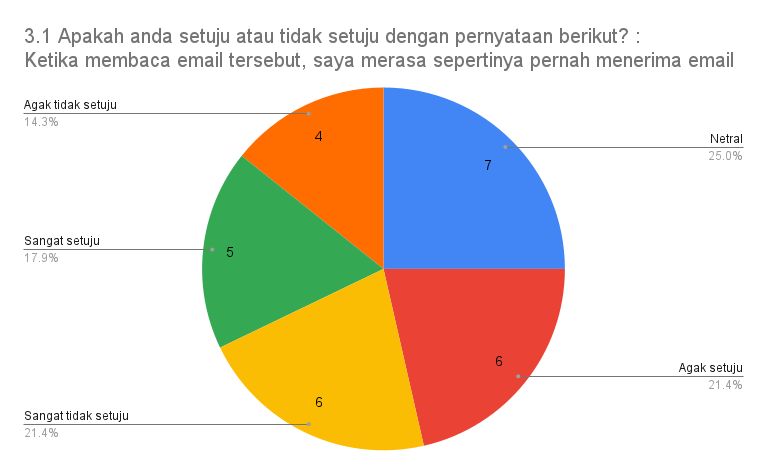
\includegraphics[width=0.5\textwidth]{image/3.1.png}
  \caption{hasil pertanyaan 3.1}
  \label{fig:pertanyaan_3.1}
\end{figure}

Fakta ini bisa membantu maupun menghambat deteksi phishing. Di satu sisi,
karena email tersebut familiar, orang dapat dengan mudah menerimanya
dan mungkin tidak membacanya dengan sangat teliti. Di
sisi lain, seperti yang ditunjukkan oleh Wash \cite{tigaempat}, ketika email
mirip dengan email lain di masa lalu, maka mungkin terbentuk ekspektasi
tentang apa yang tipikal dalam email-email sebelumnya, dan kemudian
membandingkan email ini dengan email-email sebelumnya yang serupa dan
memperhatikan lebih banyak hal yang berbeda atau salah tentang email ini.

Meskipun responden melaporkan menerima email yang mirip dengan email
mencurigakan, email mencurigakan tersebut bukanlah email yang tipikal. 71\%
responden memilih "agak setuju" atau "sangat setuju" tentang pernyataan "Pesan
email ini tampak berbeda dari pesan email yang biasanya saya terima.". Sisanya 
7\% menyatakan tidak setuju dan 21\% menyatakan netral.

\begin{figure}[h!]
  \centering
  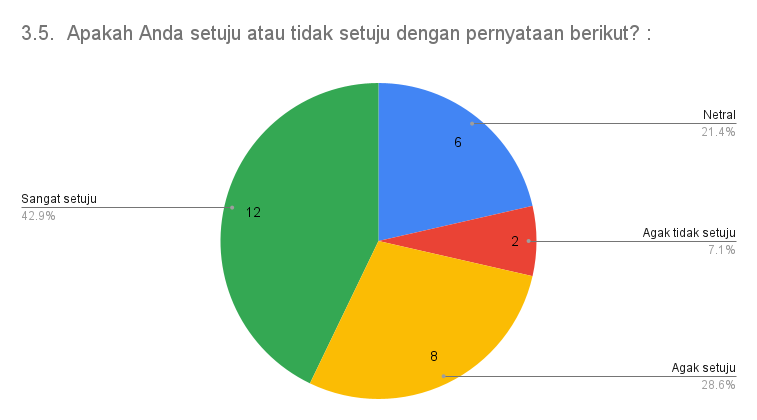
\includegraphics[width=0.5\textwidth]{image/3.5.png}
  \caption{hasil pertanyaan 3.5}
  \label{fig:pertanyaan_3.5}
\end{figure}

Menggabungkan temuan-temuan ini, email mencurigakan yang diingat orang umumnya
adalah email yang tidak diharapkan, berbeda dari email yang biasanya diterima,
tetapi sering kali mirip dengan email lain yang pernah diterima sebelumnya.
Perasaan bahwa sebuah email mencurigakan, atau tidak diharapkan, mewakili
intuisi, atau "perasaan intuitif" tentang sebuah email, dan intuisi semacam itu
sering kali merupakan aspek penting dari pengambilan keputusan manusia
\cite{satudelapan}. Hanya 3\% responden yang ingat pernah menerima email dari
pengirim ini sebelumnya. Sisanya baik tidak pernah menerima email dari pengirim
tersebut (74\%) atau tidak yakin (18\%). Jadi meskipun email tersebut terasa
familiar, pengirimnya umumnya tidak. 

\begin{figure}[h!]
  \centering
  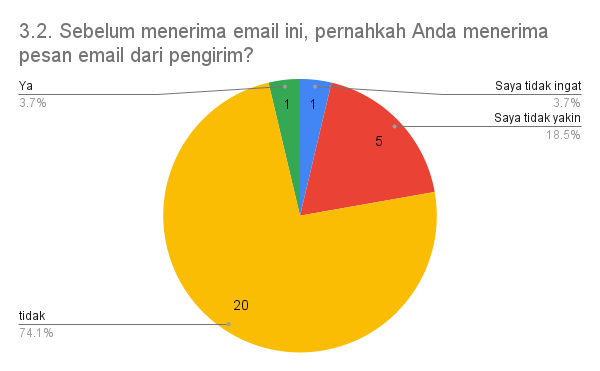
\includegraphics[width=0.5\textwidth]{image/3.2.png}
  \caption{hasil pertanyaan 3.2}
  \label{fig:pertanyaan_3.2}
\end{figure}

Lebih mencolok lagi, hanya 15\% responden
yang benar-benar pernah berinteraksi dengan pengirim sebelum membaca email ini, 14\% responden
tidak ingat dengan pengirim, dan 67\% responden menyatakan tidak pernah berinteraksi dengan pengirim
sebelumnya. Ini menunjukkan bahwa orang awam non IT mengingat dan memperhatikan dengan
siapa mereka berinteraksi melalui email dan bahwa informasi ini penting bagi
mereka saat memproses email baru.

\subsection{Request}

Definisi "phishing" dalam makalah ini adalah pesan (email) yang berpura-pura
menjadi sesuatu yang bukan sebenarnya, untuk membuat pengguna melakukan sesuatu
yang biasanya tidak akan mereka lakukan. Bagian kedua dari definisi tersebut
penting; phishing bukan hanya email palsu, tetapi email palsu yang meminta
tindakan.

Kami ingin melihat jenis tindakan apa yang diminta dalam email mencurigakan
yang diterima dan diingat oleh orang-orang. Kami bertanya kepada responden
apakah email tersebut meminta mereka melakukan salah satu dari serangkaian
tindakan umum. Tindakan yang paling umum diminta adalah mengklik tautan, yang
diminta dalam 57\% email yang dilaporkan. Ini tidak mengherankan, karena ini
adalah email phishing yang stereotip, meskipun jika ada kejutan, itu adalah
bahwa lebih dari 40\% responden tidak mengingat permintaan tautan. Hanya 19\%
email yang dilaporkan meminta pengguna untuk membuka lampiran.

46\% email meminta penerima untuk merespons email dengan beberapa jenis informasi. 
Artinya, alih-alih menggunakan halaman web untuk mengumpulkan informasi atau 
melampirkan kode berbahaya ke email, email tersebut meminta tanggapan. Menanggapi email adalah aktivitas yang sangat normal dan sehari-hari.

Hampir sepertiga email, atau 32\% email, meminta pengguna untuk mengambil
tindakan di luar konteks email. 

Sebagian besar ringkasan phishing berfokus pada cara teknis untuk mengumpulkan
informasi (tautan berbahaya, lampiran malware) \cite{tigadua}, tetapi ini
menunjukkan bahwa kita juga harus memeriksa cara non-teknis seperti hanya
membalas email. Insiden-insiden yang meminta tanggapan atau tindakan di luar
email ini adalah pengingat penting bahwa email adalah bagian kecil dari sistem
kerja yang lebih besar, dan bahwa email sering kali menjadi pemicu untuk jenis
pekerjaan lain yang harus dilakukan. Sistem anti-phishing tidak bisa hanya
fokus pada email; mereka juga perlu mengawasi pekerjaan non-email lain yang
dilakukan orang sebagai respons terhadap email.

Menariknya, 94\% responden mampu mengidentifikasi setidaknya satu tindakan yang
diminta oleh email mencurigakan. Meminta tindakan adalah bagian dari definisi
phishing karena tindakan inilah yang paling diminati oleh penyerang. Kabar
baiknya adalah bahwa pengguna tampaknya cukup memperhatikan tindakan apa yang
diminta, yang berarti ini adalah sesuatu yang selalu ada dalam semua email
phishing, dan juga sesuatu yang pengguna pandai mengidentifikasi, yang
menjadikannya tempat yang baik untuk fokus pelatihan.

\subsection{Suspecting}
Definisi phishing kami mencakup bahwa email tersebut adalah penipuan — baik
secara eksplisit berbohong atau berbohong dengan menghilangkan beberapa aspek
penting dari email tersebut. Namun, untuk menjadi curiga terhadap email
tersebut, tidak cukup hanya memperhatikan aspek-aspek email tersebut. Penerima
email juga harus mencurigai bahwa ada sesuatu yang tidak beres dengan email
tersebut.

Kami bertanya kepada responden tentang setiap bagian dari email dan apakah itu
terasa normal atau terasa "aneh" dengan cara tertentu. 59\% responden
melaporkan bahwa baris subjek email terasa "aneh" dengan cara tertentu. 70\%
responden melaporkan bahwa informasi pengirim terasa "aneh", dan 75\% responden
mengatakan bahwa isi email "aneh" dengan cara tertentu. Ini menunjukkan bahwa
ketiga aspek email dapat memberikan petunjuk penting kepada pengguna akhir
bahwa email tersebut mungkin phishing, meskipun isi (konten) email cenderung
lebih membantu pengguna.

Ketika seorang responden merasa bahwa pengirimnya aneh, mereka sekitar dua kali
lebih mungkin menunjukkan bahwa alamat email terasa aneh daripada menunjukkan
bahwa nama pengirim adalah hal yang terasa salah. Namun, seperti yang
ditunjukkan oleh cerita P99, nama juga bisa menjadi penting:

\textbf{Cerita P99}: \textit{Saat menjelajahi akun email saya, saya melihat email yang tampak palsu dari apa yang seharusnya adalah Administrasi Jaminan Sosial.

  Kecuali administrasi diganti dengan biro & segera saya tahu itu palsu. Saya
  dengan sopan menarik tempat sampah kecil untuk sesi penghapusan yang baik. Saya
  biasanya tidak membuka apa pun yang dianggap terlalu bagus untuk menjadi
  kenyataan atau palsu atau sebaliknya.}

Ketika seorang responden merasa bahwa isi email terasa aneh, kami memberikan
sejumlah opsi kepada mereka untuk menunjukkan apa yang terasa aneh dalam isi
email tersebut. 32\% responden menunjukkan bahwa isi email mencakup kesalahan
ketik yang tidak terduga atau masalah serupa lainnya. 28\% menunjukkan bahwa
isi email mencakup sesuatu yang aneh yang biasanya tidak terlihat dalam email
seperti ini. Kedua aspek ini menunjukkan bahwa kesalahan ketik pasti memicu
kecurigaan, tetapi aspek aneh lainnya dari email hampir sama umum sebagai
pemicu.

15\% menunjukkan bahwa email tersebut kehilangan sesuatu yang penting. 14\% menunjukkan bahwa email tersebut mencakup lebih sedikit informasi daripada yang mereka harapkan. Dan hanya 7\% yang menunjukkan bahwa email tersebut mencakup lebih banyak informasi daripada yang mereka harapkan. Bagi responden kami, email phishing yang mencakup lebih sedikit informasi atau kehilangan sesuatu memicu kecurigaan jauh lebih sering daripada mencakup terlalu banyak informasi. Ini berarti bahwa bagi pengguna akhir non-ahli, ekspektasi mereka tentang seberapa banyak informasi yang biasanya ada dalam email di kotak masuk mereka adalah aspek penting dari mencurigai bahwa email tersebut mungkin phishing.

\subsection{Investigating}

Wash \cite{tigaempat} menunjukkan bahwa orang jarang langsung beralih dari
memperlakukan email sebagai email asli menjadi percaya bahwa itu adalah email
phishing. Sebaliknya, ada tahap perantara yang disebut "kecurigaan." Ketika
seseorang curiga terhadap email, mereka tidak yakin apakah itu sah atau
penipuan. Selama tahap kecurigaan ini, Wash \cite{tigaempat} menggambarkan
orang-orang mengambil langkah-langkah investigasi untuk mengetahui apakah email
tersebut sah atau tidak.

Kami bertanya kepada responden tentang investigasi yang mereka lakukan terhadap
email mencurigakan mereka. 24\% responden menunjukkan bahwa mereka tidak
melakukan investigasi apa pun, dan tambahan 3\% tidak ingat apakah mereka
melakukannya. Artinya, 73\% responden melakukan setidaknya satu langkah
tambahan untuk menyelidiki email tersebut untuk menentukan apakah itu sah atau
tidak.

Langkah investigasi yang paling umum dilakukan adalah melihat lebih dekat
alamat email. 36\% responden dalam studi ini menunjukkan bahwa mereka melakukan
ini. Melihat alamat email tampaknya menjadi langkah sehari-hari yang penting
yang dicoba oleh pengguna non-ahli ketika mereka curiga terhadap email.

Cerita P66: Sebuah email masuk dari Paypal yang menjelaskan bahwa sebuah
langganan telah dibeli dengan jumlah dan nama perusahaan/orang. Saya belum
pernah melihat atau mendengar pihak yang disebutkan dan pada awalnya mengira
itu mungkin email yang sah. Setelah mempertimbangkan untuk mengklik tautan
untuk masuk ke Paypal dan menghentikan transaksi, saya mengarahkan kursor ke
informasi pengirim dan melihat alamat email tidak ada hubungannya dengan
informasi kontak PayPal.

Hanya 12\% responden yang menunjukkan bahwa mereka melihat lebih dekat pada
tautan dalam email. 7\% mengarahkan kursor ke tautan untuk melihat ke mana
arahnya, dan 5\% benar-benar mengklik tautan untuk melihat ke mana arahnya.
Investigasi tautan sering disebutkan dalam banyak pelatihan phishing, dan
mengecewakan bahwa hanya 12\% responden yang menyelidiki tautan. Sangat
mengecewakan bahwa lebih dari sepertiga dari responden tersebut mengklik tautan
sebagai langkah investigasi.

Di sisi lain, 16\% responden melaporkan melihat header email. Ini lebih umum
daripada yang kami harapkan.

\subsubsection{Investigating outside of the email}

Seperti disebutkan di atas, email sering kali hanya merupakan bagian kecil dari
sistem yang lebih besar. Selama investigasi, dimungkinkan untuk melihat di luar
email untuk mendapatkan informasi tambahan yang dapat membantu dalam
pengambilan keputusan. Dalam satu metode umum, 18\% responden melaporkan
mencari pendapat kedua tentang email tersebut dan bertanya kepada orang lain.

Kami secara khusus menanyakan kepada responden tentang langkah-langkah yang
mereka ambil untuk mempelajari lebih lanjut tentang pengirim email yang
diklaim. 82\% responden melaporkan bahwa mereka tidak mengambil langkah apa pun
untuk mempelajari lebih lanjut tentang pengirim, tetapi 18\% sisanya
melakukannya. 9\% pergi ke situs web pengirim yang diklaim untuk mendapatkan
lebih banyak informasi tentang email tersebut. 6\% mencoba menghubungi pengirim
melalui telepon. Dan 1\% berbicara dengan pengirim secara langsung, seperti
P220:

Cerita P220: Saya mendapat email dari akun email kerja saya dari apa yang saya
kira adalah rekan kerja saya. Isi email tersebut ditulis dengan kata-kata yang
aneh dan meminta saya untuk mengklik tautan yang mencurigakan. Saya melihat
lebih dekat pada alamat email yang mengirimkannya dan ternyata tidak
benar-benar sesuai dengan alamat email kerja saya. Saya pergi ke orang yang
saya kira adalah pengirim secara langsung dan bertanya apakah dia mengirim
email tersebut. Dia mengatakan tidak dan saya langsung menghapus email
tersebut.

Terlalu banyak pelatihan phishing yang berfokus pada mengajarkan orang untuk
menyelidiki email mencurigakan dengan melihat fitur-fitur internal email,
seperti alamat email pengirim dan tautan [19,30]. Mengejutkan bahwa sebanyak
18\% responden kami mengambil langkah investigasi di luar email.

\subsection{Deciding}

Wash \cite{tigaempat} menemukan bahwa setelah menyelidiki email, para ahli
dalam penelitiannya sering kali membuat keputusan akhir tentang apakah email
tersebut sah atau phishing. Kami bertanya kepada responden kami apakah mereka
membuat keputusan akhir, dan jika ya, apa keputusan tersebut. 80\% responden
membuat keputusan akhir, dan hampir semua dari mereka memutuskan bahwa email
tersebut pasti tidak aman (78\% tidak aman, 2\% aman). Sisanya 20\% masih tidak
yakin (17\%) atau tidak ingat apakah mereka membuat keputusan (3\%).

Kami bertanya kepada responden seberapa yakin mereka dengan keputusan akhir
mereka pada skala 0 hingga 10. 69\% responden memilih opsi keyakinan tertinggi
(10), dan rata-rata keyakinan adalah 8,9. Responden melaporkan tingkat
keyakinan yang sangat tinggi dalam keputusan mereka tentang apakah email
tersebut aman atau tidak.

\subsection{Acting}

Setelah memutuskan apakah email tersebut sah atau phishing, satu keputusan
masih tetap ada: apa yang harus dilakukan dengan email tersebut? Tindakan yang
paling umum adalah menghapus email tersebut. 78\% responden melaporkan bahwa
mereka menghapus email tersebut dan melanjutkan setelah memutuskan bahwa email
tersebut tidak aman. 32\% menunjukkan bahwa mereka mengklik tombol di antarmuka
mereka untuk melaporkan email sebagai spam atau phishing. Hanya 4\% yang
membiarkannya di kotak masuk mereka.

Survei hanya menanyakan tentang tindakan yang kami ketahui sebelumnya. Dalam
pengkodean manual, kami dapat mengkodekan lebih banyak tindakan. 43\% responden
menyebutkan menghapus email, dan 15\% menyebutkan mengklik tombol untuk
menandai sebagai spam atau phishing. Selain itu, 9\% membahas melaporkannya ke
pihak berwenang dengan cara lain, seperti menelepon meja bantuan IT.

32\% secara eksplisit menyebutkan "tindakan negatif": bahwa mereka
sengaja memilih untuk tidak melakukan sesuatu (seperti membuka email,
atau merespons). Tindakan negatif ini sering kali sangat kuat
dinyatakan, dan responden tampaknya merasa kuat tentang mereka,
sering menggunakan bahasa yang menggambarkan hal-hal buruk untuk membenarkan tidak melakukan
hal-hal di masa depan. Pertimbangkan, misalnya, bagaimana P115 membenarkan
tidak menjawab panggilan telepon:

\textbf{Cerita P115}: \textit{Komputer dimatikan karena akses yang tidak pantas ke situs web yang berpotensi berbahaya. Saya diberitahu bahwa saya harus membayar denda sebesar \$200 untuk mendapatkan akses ke komputer saya. Saya menerima panggilan telepon tentang pergi ke toko lokal untuk membeli kartu hadiah. Saya sampai pergi ke toko untuk membeli kartu hadiah dan saat checkout, petugas di kasir memberi tahu saya bahwa saya sedang ditipu dan tidak membeli kartu-kartu ini. Sementara itu, saya memiliki saluran terbuka dengan penipu ini, yang segera saya tutup. Setelah tiba di rumah, saya terus menerima panggilan telepon dari orang ini, yang tidak pernah saya ajak bicara lagi.}

Tambahan 9\% responden melaporkan mengambil tindakan pencegahan yang lebih
ketat di masa depan, seperti menginstal pemindai virus atau lebih berhati-hati
dengan email.

Orang juga memiliki reaksi emosional terhadap email tersebut. Kami bertanya
kepada responden tentang pengalaman mereka terhadap serangkaian emosi, termasuk
"gugup," "takut," "teror," "kecemasan," "khawatir," dan "cemas". Semua emosi
memiliki skor yang sangat rendah, dan tidak ada emosi yang rata-rata lebih dari
2,2 dari 5. Meskipun tidak aman, email-email ini tidak menimbulkan emosi yang
kuat dari responden kami. Pelatihan phishing sebelumnya, terutama yang berasal
dari Protection Motivation Theory, telah menggunakan ajakan ketakutan untuk
memotivasi pengguna \cite{lima,duanol}. Berdasarkan data ini, email phishing
umumnya tidak menyebabkan emosi yang kuat, dan ini bisa menjelaskan mengapa
ajakan ketakutan tidak memotivasi perubahan perilaku \cite{enam}.

\section{Discussion}

\subsubsection{Humans Identify Phishing Differently}
Sistem email modern melibatkan beberapa lapisan perlindungan terhadap serangan
phishing. Banyak pengirim email menyertakan pemeriksaan phishing saat email
dikirim. Sebagian besar sistem email menyertakan setidaknya satu, dan sering
kali lebih dari satu sistem teknis yang menyaring email yang diyakini sebagai
spam atau phishing. Banyak dari sistem ini juga memberi label email sebagai
kemungkinan phishing, sebagai peringatan kepada pengguna (misalnya, sistem
email Google \cite{dualima}). Dan pengguna akhir membaca email dan membuat
penentuan legitimasi mereka sendiri.

Model Swiss Cheese dari Reason tentang penyaringan \cite{duadelapan}
menunjukkan bahwa ketika ada rantai filter seperti ini, filter bekerja paling
baik ketika setiap filter bekerja pada prinsip yang berbeda atau menggunakan
informasi yang berbeda dari filter lain dalam rantai. Jika dua filter
menggunakan informasi yang sama (misalnya, alamat email pengirim) dengan cara
yang sama, maka lubang di keju akan sejajar dan email berbahaya yang lolos dari
satu filter juga kemungkinan besar akan lolos dari yang lain. Namun, jika dua
filter menggunakan informasi yang berbeda, atau beroperasi pada informasi
dengan cara yang sangat berbeda, maka setiap filter kemungkinan akan menangkap
pesan yang terlewatkan oleh filter lainnya, dan menyertakan kedua filter
membuat sistem lebih tangguh terhadap serangan daripada hanya menyertakan satu.

Dalam makalah ini, kami menyajikan bukti bahwa filter terakhir ini – manusia
yang membaca email dan menentukan apakah email tersebut sah – beroperasi dengan
cara yang sangat berbeda, menggunakan pengetahuan dan kemampuan yang berbeda,
daripada hampir semua filter teknis. Kami menemukan bahwa manusia memiliki
informasi penting yang tidak dimiliki oleh filter phishing teknis. Mereka
mengandalkan keakraban mereka dengan email terkait yang diterima di masa lalu
(72\%) dan harapan mereka terhadap email yang masuk (95\%) untuk memahami dan
menjadi curiga terhadap email phishing. Pengetahuan ini sangat kontekstual dan
sangat unik bagi setiap individu dan pengalaman mereka. Selain itu, manusia
menggunakan pengetahuan mereka tentang apa yang biasa ada dalam email yang
mereka terima di masa lalu untuk melihat bagian informasi yang tidak terduga
dan hilang dalam email baru. Informasi ini sangat penting untuk mendeteksi
serangan phishing zero-day, yang jarang terdeteksi oleh solusi teknis
\cite{satudua}.

Responden kami mampu memperhatikan sifat email (misalnya 78\% memperhatikan
bahwa itu bersifat pribadi) dan akun email tempat email diterima. Ini
memerlukan pengetahuan tentang semua akun email yang dimiliki seseorang dan
jenis komunikasi yang diharapkan di setiap akun berdasarkan bagaimana dan apa
yang dipilih orang tersebut untuk menggunakan setiap akun. Sangat kompleks dan
menantang bagi filter teknis untuk memperoleh pengetahuan semacam itu dan
menerapkannya dengan tepat, kecuali mereka mengawasi individu.

Kedua, kami menemukan bahwa manusia memiliki kemampuan unik yang mereka gunakan
untuk mengidentifikasi pesan phishing, yang tidak dimiliki oleh filter teknis.
94\% responden non-ahli mampu mengidentifikasi tindakan apa yang diminta email
untuk mereka lakukan, dan lebih dari tiga perempat mengatakan mereka secara
eksplisit memperhatikan hal ini tentang email tersebut. Permintaan untuk
tindakan tidak umum menjadi bagian dari banyak filter spam dan phishing, dan
ketika ada, sering kali terbatas dalam cakupan terutama oleh masalah bahasa
(misalnya memeriksa apakah email berisi tautan ke halaman login dan
memverifikasi apakah halaman login tersebut sah \cite{duatiga}). Bahkan
non-ahli sangat peka terhadap permintaan ini dan dapat mengidentifikasinya
dengan percaya diri.

Saat menyaring, manusia juga memiliki kemampuan investigasi yang tidak dimiliki
oleh filter teknis: mereka dapat memilih untuk mengambil waktu tambahan dan
mencari lebih banyak informasi dari sumber pihak ketiga. Sejumlah responden
kami menunjukkan bahwa mereka akan meminta nasihat dari rekan kerja atau
mencoba menghubungi pengirim email yang diklaim.

Di atas adalah kemampuan dan pengetahuan yang dimiliki manusia, tetapi tidak
dimiliki oleh filter phishing teknis. Mengikuti logika Model Swiss Cheese,
mengandalkan kombinasi penyaringan manusia dan teknis lebih baik daripada hanya
mengandalkan salah satu. Dalam beberapa tahun terakhir, organisasi telah lebih
mengandalkan deteksi phishing otomatis. Temuan kami menunjukkan bahwa
mengurangi keragaman filter dapat membuat sistem rentan terhadap phishing, dan
bahwa mendekati pelatihan pengguna akhir dengan cara yang berbeda dapat
memperkuat strategi untuk mencegah kerugian dari phishing.

Banyak saran tentang phishing dalam komunitas TI melibatkan pencegahan pesan
agar tidak pernah sampai ke pengguna akhir \cite{satuempat}, daripada mencoba
mendidik pengguna akhir. Karena pengguna akhir mampu menyaring pesan dengan
cara yang sangat berbeda dari filter teknis, akan lebih berharga untuk
menghabiskan sebagian uang dan sumber daya untuk meningkatkan kemampuan
pengguna akhir untuk memiliki peran signifikan dalam mendeteksi pesan phishing.
Terlalu banyak pelatihan phishing yang berfokus pada detail teknis (seperti
parsing URL [19, 30]) atau perubahan perilaku (seperti tidak mengklik [20,
    35]), daripada mencoba memperkuat kemampuan yang unik bagi manusia. Dalam
makalah ini, kami telah menyajikan bukti beberapa pengetahuan dan kemampuan
yang dimiliki manusia yang dapat dimanfaatkan untuk meningkatkan pelatihan dan
deteksi phishing, misalnya membentuk harapan untuk email dan meminta informasi
dari orang lain.

Seperti yang ditunjukkan oleh Model Swiss Cheese, dalam serangkaian filter,
menempatkan semua sumber daya Anda ke dalam satu lapisan filter dengan
mengesampingkan yang lain menghilangkan manfaat yang Anda dapatkan dari
strategi pertahanan berlapis. Seringkali lebih baik memiliki dua filter yang
tidak sempurna yang beroperasi pada prinsip atau informasi yang berbeda
daripada memiliki satu filter yang sangat dioptimalkan tetapi terbatas.

\subsubsection{Similar to Expert Phishing Detection?}

Temuan kami juga memiliki implikasi untuk mengidentifikasi kesamaan antara
deteksi email phishing oleh pengguna ahli dan non-ahli. Wash \cite{tigaempat}
melakukan studi mendetail tentang bagaimana orang mendeteksi email phishing.
Studi tersebut dilakukan dengan para ahli IT – orang-orang dengan pelatihan IT
dan pengalaman profesional yang memungkinkan mereka untuk berhasil mendeteksi
email phishing. Kami memperluas model tersebut, dan mendasarkan banyak
pertanyaan kami pada model yang diperluas tersebut, sebagian untuk mencoba
menentukan apakah fitur-fitur dari model tersebut juga ada dalam cara non-ahli
mendeteksi phishing.

Dalam makalah ini, kami dapat memvalidasi bagian dari modelnya dengan populasi
non-ahli. Wash juga menunjukkan bahwa selain keahlian IT, menjadi pekerja
pengetahuan dapat memberikan keahlian dalam mengelola email yang relevan dengan
deteksi phishing. Sampel kami bukan ahli IT, dan juga bukan pekerja pengetahuan
yang secara konstan berurusan dengan email.

Secara khusus, kami dapat memvalidasi bahwa non-ahli memang memiliki ekspektasi
tentang apa yang seharusnya ada dalam email dan memperhatikan ketika hal-hal
tersebut berbeda. Kami juga dapat memvalidasi bahwa bahkan pada non-ahli,
perhatian orang terfokus pada apa yang diminta email untuk mereka lakukan;
hampir semua orang dalam studi kami dapat mengidentifikasi permintaan apa yang
dibuat oleh email tersebut. Kami memvalidasi bahwa non-ahli kami melaporkan
bahwa mereka sering memiliki firasat bahwa ada sesuatu yang salah dengan email
tersebut, membantu mereka menjadi curiga. Kami dapat memvalidasi bahwa orang
sering mengambil langkah eksplisit untuk menyelidiki email yang mereka anggap
mencurigakan. Dan kami dapat memvalidasi bahwa non-ahli mampu secara konklusif
memutuskan apakah email tersebut adalah email phishing atau tidak. Ini
mendukung implikasi bahwa keahlian tentang kotak masuk email seseorang adalah
aspek penting dan belum dimanfaatkan dalam pelatihan deteksi phishing.

Kami tidak dapat memvalidasi semua aspek model Wash dengan non-ahli. Secara
khusus, model Wash mencakup urutan kronologis dari tahap-tahap – pertama
pemahaman, kemudian kecurigaan, kemudian bertindak. Studi kami adalah survei
dan tidak dapat menentukan urutan kronologis dari kejadian, dan dengan
demikian, kami tidak yakin bahwa hal-hal tersebut terjadi pada non-ahli dalam
urutan yang diusulkan oleh Wash.

\subsubsection{Implications for Phishing Prevention}
Pengguna email melakukan investigasi yang kompleks terhadap email yang
mencurigakan sebelum mereka menentukan apakah email tersebut adalah phishing,
tetapi pelatihan dan teknologi saat ini tidak mendukung investigasi ini. Temuan
kami menunjukkan bahwa pelatihan phishing dapat lebih mendukung investigasi
pengguna dengan mendorong pengguna untuk menunda tindakan hingga menyelesaikan
investigasi mereka dan mendorong pengguna email untuk memanfaatkan kemampuan
rekan (seperti meminta bantuan teman). Selain itu, perusahaan yang mengirim
email dapat menyediakan dukungan gaya helpdesk untuk membantu pengguna
menentukan apakah perusahaan benar-benar mengirim email tersebut kepada
pengguna. Klien email dapat lebih mendukung investigasi dengan menyertakan
tombol "bantu saya memecahkan masalah email ini", dengan saran kontekstual
untuk investigasi.

\section{Limitations}
Makalah ini tentang orang-orang, kognisi mereka, dan bagaimana mereka berhasil
mendeteksi phishing. Ini bukan tentang email phishing. Survei bukanlah metode
yang baik untuk mengumpulkan data kebenaran dasar tentang email phishing yang
sebenarnya atau kegagalan deteksi, karena bias seleksi dan ingatan yang tidak
sempurna.

Mengingat email phishing mendorong pengingatan kejadian tertentu, memungkinkan
survei untuk menyelidiki proses yang digunakan orang untuk mendeteksi email
phishing di kotak masuk mereka. Jawaban yang kami terima hanya tentang satu
insiden spesifik ini, dan tidak selalu mewakili insiden lain yang dialami orang
tersebut; namun, di antara responden, jawaban ini mewakili berbagai jenis
insiden phishing yang dihadapi oleh non-ahli. Penelitian sebelumnya hampir
secara eksklusif berfokus pada kegagalan deteksi dan memperbaiki kegagalan
tersebut; kami sebaliknya melihat apa yang bekerja dengan baik dalam deteksi
phishing dan apa yang harus didukung.

Karena ini adalah survei, kami hanya dapat mengajukan pertanyaan rinci tentang
hal-hal yang kami ketahui sebelumnya. Kami mendasarkan pertanyaan survei kami
pada investigasi Wash tentang deteksi phishing oleh ahli \cite{tigaempat}. Kami
tidak dapat menentukan apakah non-ahli juga menggunakan metode tambahan yang
tidak ada pada ahli Wash. Artinya, kami berusaha untuk mengetahui metode ahli
mana yang juga digunakan oleh non-ahli, tetapi kami tidak dapat mempelajari
metode non-ahli yang unik untuk non-ahli. Oleh karena itu, kami tidak mengklaim
bahwa metode ini adalah deskripsi komprehensif tentang bagaimana non-ahli
mengidentifikasi phishing; sebaliknya, kami mengkarakterisasi beberapa metode
yang mereka gunakan.

\section{Conclusion}
Phishing adalah ancaman keamanan siber yang dialami banyak orang; hampir
setengah dari orang yang memenuhi syarat untuk survei kami dapat
mengidentifikasi setidaknya satu email phishing spesifik yang mereka terima.
Orang-orang ini memiliki cerita tentang pengalaman phishing yang dapat mereka
bagikan dengan orang lain, dan kami menduga cerita-cerita ini membentuk bagian
penting dari bagaimana pengguna email belajar tentang phishing.

Kami menemukan bahwa banyak teknik yang digunakan para ahli untuk
mengidentifikasi phishing \cite{tigaempat}, seperti memperhatikan
ketidaksesuaian kecil, membentuk ekspektasi tentang bagaimana email seharusnya
terlihat dan memperhatikan perbedaan dari ekspektasi tersebut, serta menjadi
curiga dan menyelidiki email lebih dekat, juga hadir dalam cara non-ahli
mendeteksi email phishing.

Kami juga menemukan bahwa banyak informasi yang digunakan non-ahli saat
mengidentifikasi phishing tidak dapat direplikasi oleh sistem deteksi phishing
teknis. Pengguna akhir mengetahui tujuan (bisnis, pribadi) dari akun email
tempat mereka menerima email, dan memperhatikan fakta tersebut. Mereka tahu
apakah email tersebut diharapkan, dan dapat membandingkannya dengan email lain
yang serupa yang pernah mereka terima di masa lalu (email phishing sering kali
terasa familiar). Selain itu, non-ahli ini memiliki kemampuan investigasi,
seperti menunda merespons email dan meminta konfirmasi atau informasi lebih
lanjut dari pengirim, yang tidak dimiliki oleh filter phishing teknis.
Menargetkan pelatihan phishing di masa depan untuk meningkatkan penggunaan
pengetahuan unik ini dan memperluas penggunaan kemampuan ini kemungkinan akan
menghasilkan peningkatan dalam perlindungan phishing.

\section*{Acknowledgments}
This should be a simple paragraph before the References to thank those individuals and institutions who have supported your work on this article.

\begin{thebibliography}{1}
  \bibliographystyle{IEEEtran}

  \bibitem{satu}
  Jeremy Bryans and Budi Arief. Security implications of structure. In Structure for Dependability: Computer-Based Systems from an Interdisciplinary Perspective, pages 217–227. Springer, 2006.

  \bibitem{dua}
  Deanna D Caputo, Shari Lawrence Pfleeger, Jesse D
  Freeman, and M Eric Johnson. Going spear phishing:
  Exploring embedded training and awareness. IEEE
  Security & Privacy, 12(1):28–38, 2013.

  \bibitem{tiga}
  Debra L. Cook, Vijay K. Gurbani, and Michael Daniluk.
  Phishwish: a simple and stateless phishing filter. Secu-
  rity and Communication Networks, 2(1):29–43, 2009.

  \bibitem{empat}
  Lorrie Faith Cranor. Can phishing be foiled? Scientific
  American, 299(6):104–111, 2008.

  \bibitem{lima}
  Nicola Davinson and Elizabeth Sillence. It won’t happen
  to me: Promoting secure behaviour among internet users.
  Computers in Human Behavior, 26(6):1739–1747, 2010.

  \bibitem{enam}
  Julie S. Downs, Mandy Holbrook, and Lorrie Faith Cra-
  nor. Behavioral response to phishing risk. In Proceed-
  ings of the Anti-Phishing Working Groups 2nd Annual
  ECrime Researchers Summit, eCrime ’07, pages 37–44,
  New York, NY, USA, 2007. Association for Computing
  Machinery.

  \bibitem{tujuh}
  Julie S Downs, Mandy B Holbrook, and Lorrie Faith
  Cranor. Decision strategies and susceptibility to phish-
  ing. In Proceedings of the second symposium on Usable
  privacy and security, pages 79–90, 2006.

  \bibitem{delapan}
  Serge Egelman, Lorrie Faith Cranor, and Jason Hong.
  You’ve been warned: An empirical study of the effective-
  ness of web browser phishing warnings. In Proceedings
  of the SIGCHI Conference on Human Factors in Com-
  puting Systems, CHI ’08, pages 1065–1074, New York,
  NY, USA, 2008. Association for Computing Machinery.

  \bibitem{sembilan}
  Ian Fette, Norman Sadeh, and Anthony Tomasic. Learn-
  ing to detect phishing emails. In Proceedings of the 16th
  International Conference on World Wide Web, WWW
  ’07, pages 649–656, New York, NY, USA, 2007. Asso-
  ciation for Computing Machinery.

  \bibitem{satunol}
  Joshua T Goodman, Paul S Rehfuss, Robert L Rounthwaite, Manav Mishra, Geoffrey J Hulten, Kenneth G Richards, Aaron H Averbuch, Anthony P Penta, and Roderict C Deyo. Phishing detection, prevention, and notification, October 16 2012. US Patent 8,291,065.

  \bibitem{satusatu}
  The Radicati Group, ``Email statistics report 2019-2023 executive summary,'' Technical report, The Radicati Group, 2019.

  \bibitem{satudua}
  Ryan Heartfield and George Loukas. A taxonomy of
  attacks and a survey of defence mechanisms for seman-
  tic social engineering attacks. ACM Computing Surveys
  (CSUR), 48(3):1–39, 2015.

  \bibitem{satutiga}
  Thorsten Holz, Christian Gorecki, Konrad Rieck, and
  Felix C Freiling. Measuring and detecting fast-flux ser-
  vice networks. In The Network and Distributed System
  Security Symposium (NDSS), 2008.

  \bibitem{satuempat}
  Jason Hong. The state of phishing attacks. Communications of the ACM, 55(1):74, Jan 2012.

  \bibitem{satulima}
  Scott D Johnson, Jeffrey W Flesher, and Shih-Ping
  Chung. Understanding troubleshooting styles to im-
  prove training methods. In American Vocational Associ-
  ation Convention. ERIC, Dec 1995.

  \bibitem{satuenam}
  Y. Joshi, S. Saklikar, D. Das, and S. Saha. Phishguard:
  A browser plug-in for protection from phishing. In
  2008 2nd International Conference on Internet Multimedia Services Architecture and Applications, pages 1–6,
  2008.

  \bibitem{satutujuh}
  Mahmoud Khonji, Youssef Iraqi, and Andrew Jones.
  Phishing detection: a literature survey. IEEE Communications Surveys & Tutorials, 15(4):2091–2121, 2013.

  \bibitem{satudelapan}
  Gary Klein. Sources of Power: How People Make Decisions. MIT Press, 1998.

  \bibitem{satusembilan}
  Ponnurangam Kumaraguru, Steve Sheng, Alessandro
  Acquisti, Lorrie Faith Cranor, and Jason Hong. Teach-
  ing johnny not to fall for phish. ACM Transactions on
  Internet Technology (TOIT), 10(2):1–31, 2010.

  \bibitem{duanol}
  Robert LaRose, Nora J. Rifon, and Richard Enbody. Pro-
  moting personal responsibility for internet safety. Com-
  munications of the ACM, 51(3):71–76, March 2008.

  \bibitem{duasatu}
  Eric Lipton, David E Sanger, and Scott Shane. The Perfect Weapon: How Russian Cyberpower Invaded the U.S. The New York Times, dec 2016.

  \bibitem{duadua}
  MacEwan University. University Discovers Online Fraud. Press Release, 2017. https://www.macewan.ca/wcm/MacEwanNews/PHISHING\_ATTACK.

  \bibitem{duatiga}
  L. A. T. Nguyen, B. L. To, H. K. Nguyen, and M. H.
  Nguyen. A novel approach for phishing detection using
  url-based heuristic. In 2014 International Conference
  on Computing, Management and Telecommunications
  (ComManTel), pages 298–303, 2014.

  \bibitem{duaempat}
  US Bureau of Labor Statistics. Employment–
  population ratio, Retrieved Feb, 2021. https:
  //www.bls.gov/charts/employment-situation/
  employment-population-ratio.htm.

  \bibitem{dualima}
  Rob Pegoraro. We keep falling for phishing emails,
  and google just revealed why. Fast Company,
  2019. https://www.fastcompany.com/90387855/
  we-keep-falling-for-phishing-emails-and-
  google-just-revealed-why.

  \bibitem{duaenam}
  Justin Petelka, Yixin Zou, and Florian Schaub. Put your
  warning where your link is: Improving and evaluating
  email phishing warnings. In Proceedings of the 2019
  CHI Conference on Human Factors in Computing Sys-
  tems, CHI ’19, pages 1–15, New York, NY, USA, 2019.
  Association for Computing Machinery.

  \bibitem{duatujuh}
  Emilee Rader, Rick Wash, and Brandon Brooks. Stories
  as informal lessons about security. In Proceedings of
  the Eighth Symposium on Usable Privacy and Security
  (SOUPS), pages 1–17, 2012.

  \bibitem{duadelapan}
  James Reason. Human Error. Cambridge University
  Press, 1990.

  \bibitem{duasembilan}
  Ozgur Koray Sahingoz, Ebubekir Buber, Onder Demir,
  and Banu Diri. Machine learning based phishing de-
  tection from urls. Expert Systems with Applications,
  117:345 – 357, 2019.

  \bibitem{tiganol}
  Steve Sheng, Bryant Magnien, Ponnurangam Ku-
  maraguru, Alessandro Acquisti, Lorrie Faith Cranor, Ja-
  son Hong, and Elizabeth Nunge. Anti-phishing phil: the
  design and evaluation of a game that teaches people not
  to fall for phish. In Proceedings of the 3rd Symposium
  on Usable Privacy and Security (SOUPS), pages 88–99,
  2007.

  \bibitem{tigasatu}
  Rebecca Smith. How a U.S. Utility Got Hacked. Wall Street Journal, Dec 2016.

  \bibitem{tigadua}
  Symantec. Internet Security Threat Report. Technical Report February, 2019.

  \bibitem{tigatiga}
  Verizon. 2019 Data Breach Investigations Report. Technical report, 2019.

  \bibitem{tigaempat}
  Rick Wash. How experts detect phishing scam emails. Proceedings of the ACM: Human Computer Interaction, CSCW(160), October 2020.

  \bibitem{tigalima}
  Rick Wash and Molly M Cooper. Who provides phish-
  ing training? facts, stories, and people like me. In Pro-
  ceedings of the 2018 CHI Conference on Human Factors
  in Computing Systems, pages 1–12, 2018.

  \bibitem{tigaenam}
  Steve Whittaker, Victoria Bellotti, and Jacek Gwizdka.
  Email in personal information management. Communi-
  cations of the ACM, 49(1):68–73, January 2006.

  \bibitem{tigatujuh}
  Weining Yang, Aiping Xiong, Jing Chen, Robert W.
  Proctor, and Ninghui Li. Use of phishing training to
  improve security warning compliance: Evidence from a
  field experiment. In Proceedings of the Hot Topics in Sci-
  ence of Security: Symposium and Bootcamp, HoTSoS,
  pages 52–61, New York, NY, USA, 2017. Association
  for Computing Machinery.

  \bibitem{ref10}
  Wash, R., Nthala, N., & Rader, E. (2021). Knowledge and capabilities that {Non-Expert} users bring to phishing detection. In \textit{Seventeenth Symposium on Usable Privacy and Security (SOUPS 2021)} (pp. 377-396).

\end{thebibliography}

\newpage

\section{Biography Section}
If you have an EPS/PDF photo (graphicx package needed), extra braces are needed
around the contents of the optional argument to biography to prevent the LaTeX
parser from getting confused when it sees the complicated
$\backslash${\tt{includegraphics}} command within an optional argument. (You
can create your own custom macro containing the
$\backslash${\tt{includegraphics}} command to make things simpler here.)

\vspace{11pt}

\bf{If you include a photo:}\vspace{-33pt}
\begin{IEEEbiography}[{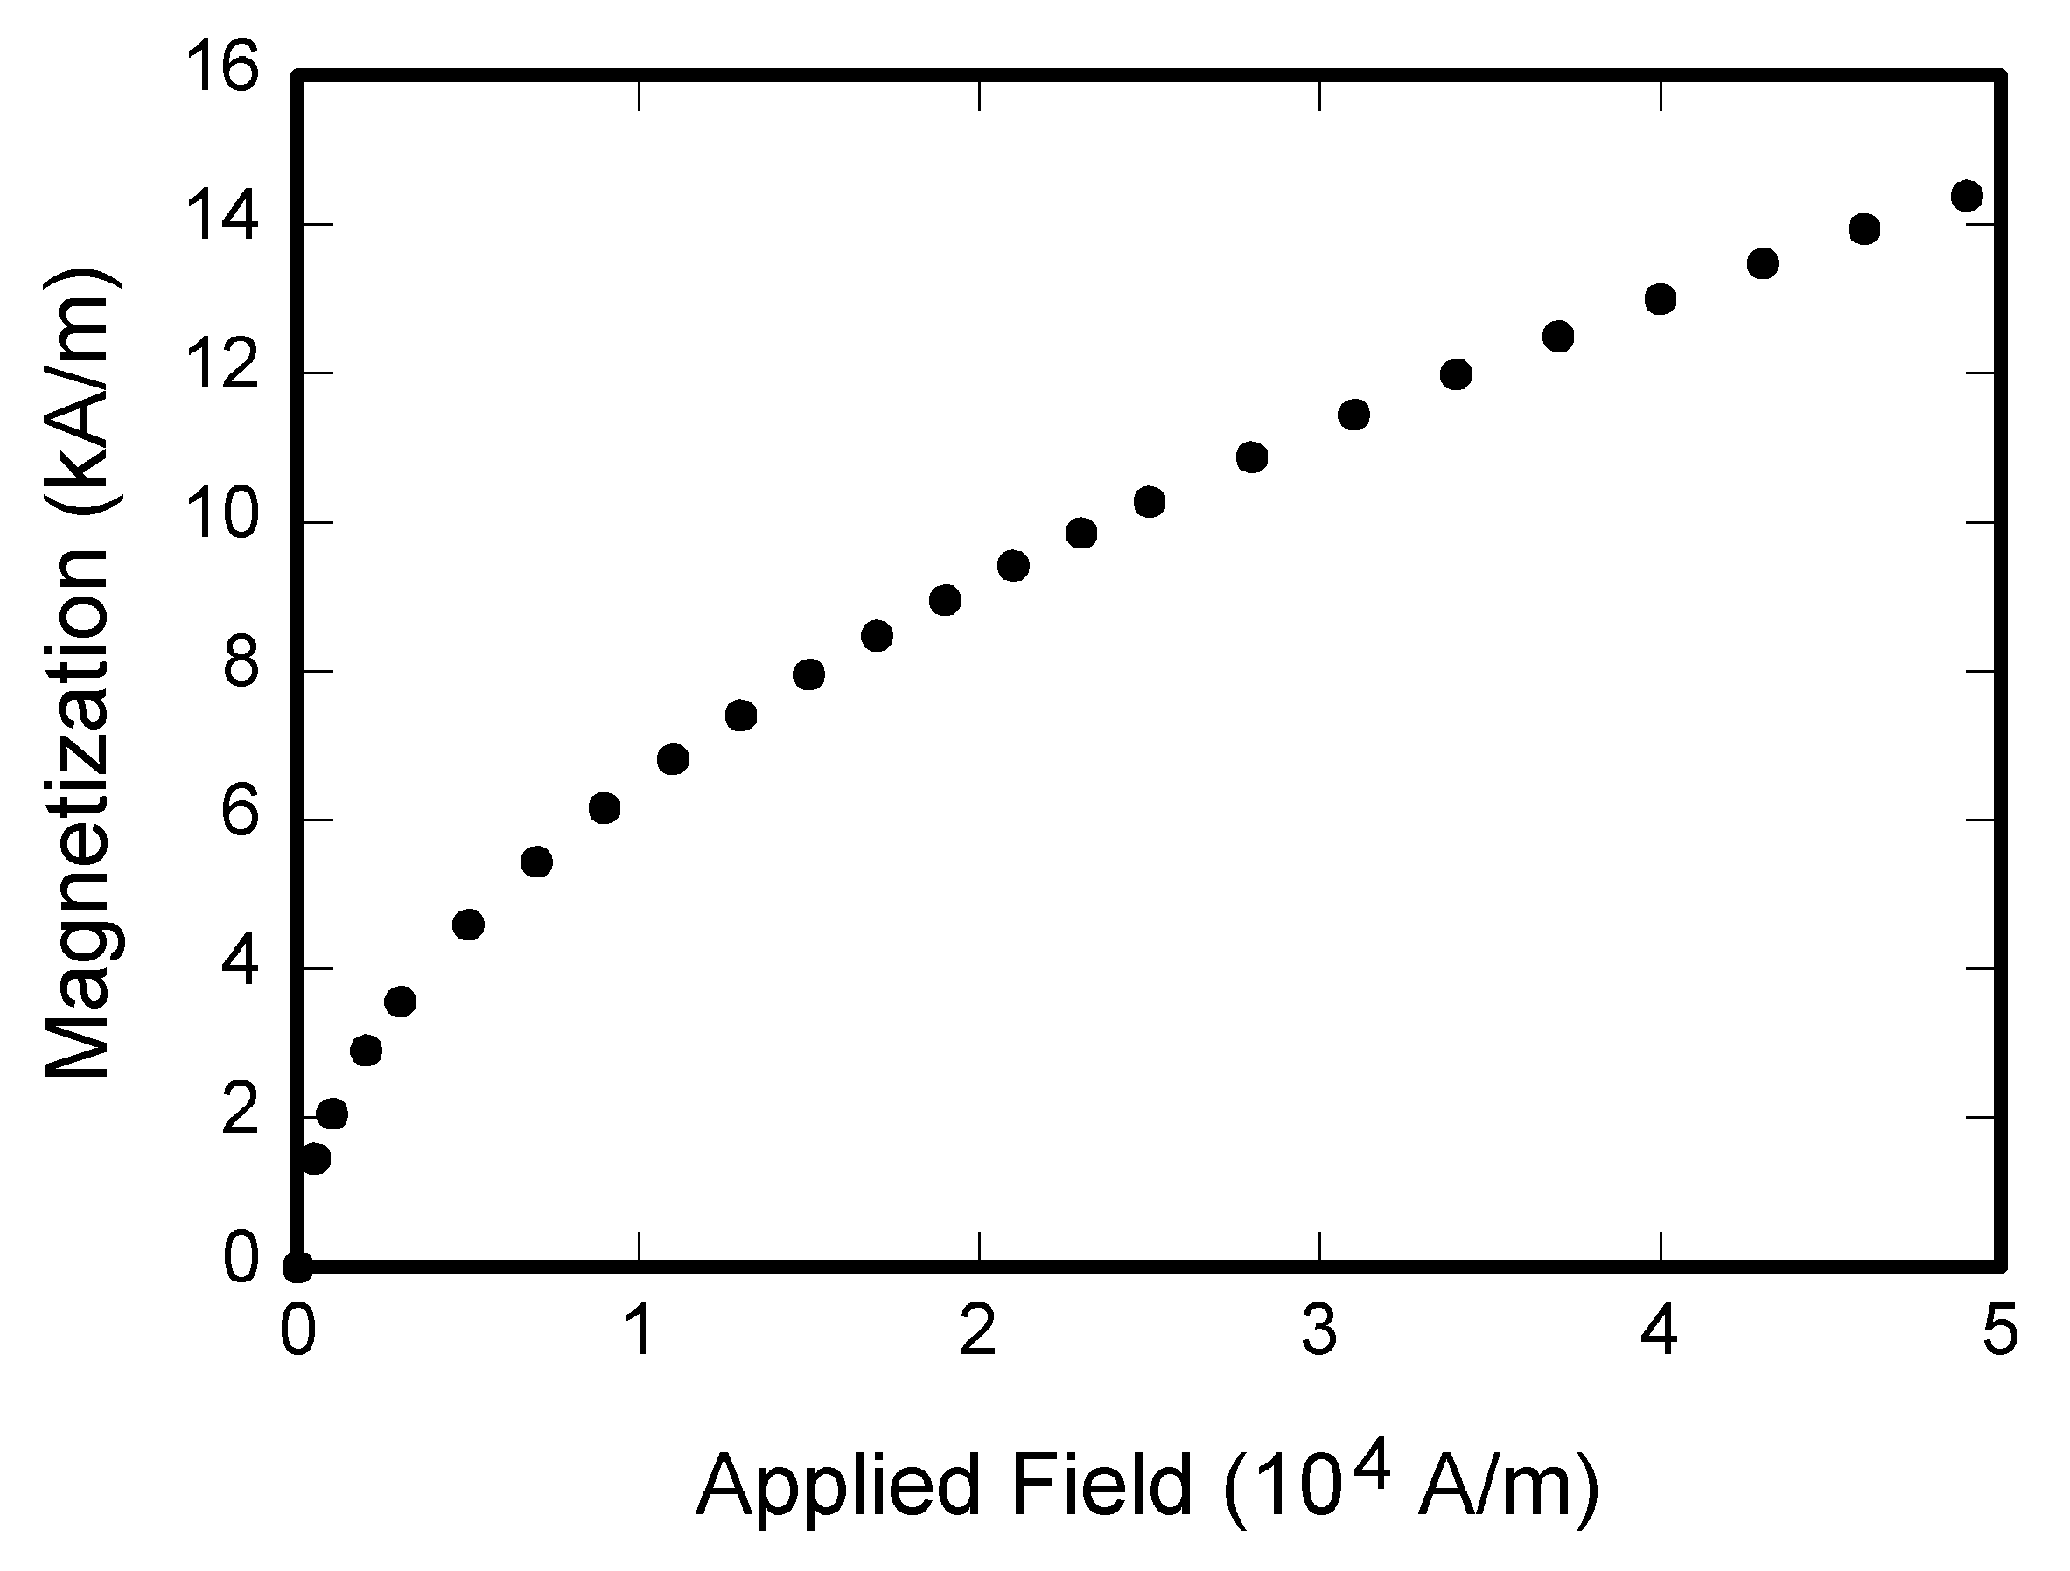
\includegraphics[width=1in,height=1.25in,clip,keepaspectratio]{fig1}}]{Michael Shell}
  Use $\backslash${\tt{begin\{IEEEbiography\}}} and then for the 1st argument use $\backslash${\tt{includegraphics}} to declare and link the author photo.
  Use the author name as the 3rd argument followed by the biography text.
\end{IEEEbiography}

\vspace{11pt}

\bf{If you will not include a photo:}\vspace{-33pt}
\begin{IEEEbiographynophoto}{John Doe}
  Use $\backslash${\tt{begin\{IEEEbiographynophoto\}}} and the author name as the argument followed by the biography text.
\end{IEEEbiographynophoto}

\vfill

\end{document}

